\chapter{Collektive: aggregate programming in pure Kotlin}\label{chapter:collektive}
The name given to the project is \textbf{Collektive}\footnote{\url{https://github.com/ElisaTronetti/collektive}}, which emphasize the aggregate programming aim to dispose of numerous devices that work together to achieve a certain goal. Moreover, the name contains the term \textbf{`kt'}, which refers to the development in Kotlin.

The goal of Collektive is to provide to the user a minimal DSL that makes it possible to create aggregate programs transparently. It is necessary to keep in mind that the solution needs to respect these requirements:
\begin{itemize}
    \item \textbf{Transparency}: refers to the clear and concise information it provides about how the underlying system behaves, such as data processing, storage, and communication between nodes. Transparency helps to reduce complexity, making it easier to understand and maintain large and complex systems;
    \item \textbf{Minimality}: the goal is to design it with the fewest possible constructs and abstractions while still offering the required functionalities. This reduces the complexity of the system, making it easier to maintain and debug, and lowers the overhead associated with using the DSL, which is particularly important for systems that require high performance and scalability;
    \item \textbf{Portability}: refers to its ability to run on various platforms and environments, including different operating systems, cloud platforms, and hardware architectures. This enables systems built with the DSL to be easily deployed and run in different environments, which is crucial for systems requiring deployment in multiple locations or scalability to meet changing demands.
\end{itemize}

The following sections are organized in order to present in details the project developed. Specifically, Section~\ref{section:technology_choices} discuss the main technological choice involved in the development of the DSL, in Section~\ref{section:project_structure} is shown the project structure, in Section~\ref{section:dsl} is analyzed in details the DSL created. Then, Section~\ref{section:usage_example} presents the final result and how the DSL can be used, and Section~\ref{section:validation} is used to highlight the validation methods applied to test the correct behavior of the project developed.

\section{Technology}\label{section:technology_choices}
This section presents the main technological choice taken regarding the development of the DSL, in order to meet the requirements cited previously.\newline
It is important to achieve a certain level of portability, specifically for devices running on JVM, JS and Kotlin Native platforms, which makes also possible  to gain interoperability between different targets. Moreover, an ideal solution would not require writing the DSL code in three different programming languages to match the required platforms.\newline
For the reasons just presented, the choice made for this project development is \textbf{Kotlin Multiplatform}.

\subsection{Kotlin Multiplatform}
Kotlin Multiplatform technology is specifically designed to streamline the development process for cross-platform projects.\newline
It achieves this by minimizing the amount of time developers spend writing and maintaining identical code for different platforms. This approach saves valuable resources and time, as the code can be written once and used across multiple platforms.

Kotlin Multiplatform allows to write code in the Kotlin programming language and use it across multiple platforms, including Android, iOS, web, and desktop.
\begin{figure}[!ht]
    \centering
    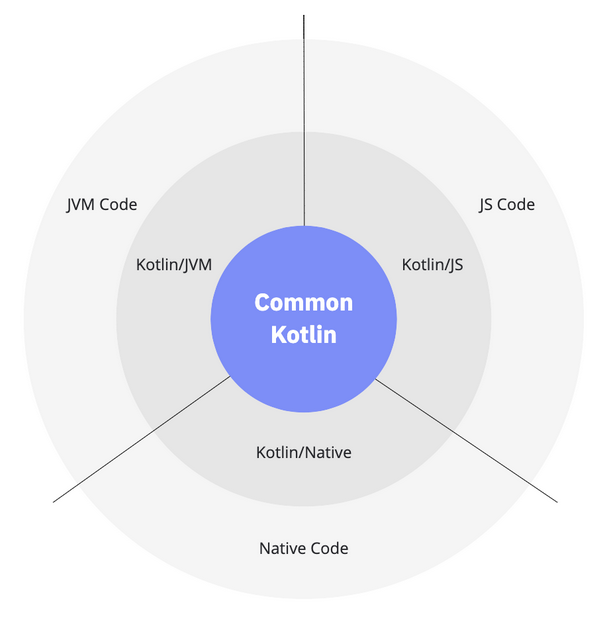
\includegraphics[scale=0.9]{document/chapters/4-collektive/images/kotlin_multiplatform_code.png}
    \caption{How Kotlin Multiplatform works}
    \label{fig:km_code_work}
\end{figure}
As can be seen in Figure~\ref{fig:km_code_work}\footnote{\url{https://kotlinlang.org/docs/multiplatform.html} \label{km_footnote}}, Kotlin Multiplatform code behaves in the following way\footref{km_footnote}:
\begin{itemize}
    \item \textbf{Common Kotlin}: the code written in common Kotlin can be used across multiple platforms without requiring modifications. This code can include business logic, data models, and other non-platform-specific functionalities. Common code can rely on a set of libraries that are available for Kotlin Multiplatform and that cover everyday tasks, such as serializations or coroutines;
    \item \textbf{Platform-specific versions of Kotlin}: this refers to \textbf{Kotlin/JVM}, \textbf{Kotlin/JS} and \textbf{Kotlin/Native}, which include extensions to the Kotlin language, allowing developers to use platform-specific APIs, features and tools;
    \item \textbf{Platform native code}: finally, through these platforms it is possible to access the platform native code (JVM, JS and Native), with the possibility to use all the native features.
\end{itemize}

The way that Kotlin Multiplatform avoid the necessity to write and maintain the same code over and over again for all the targeted platforms, is by providing the possibility to share the same code across multiple platforms.\newline
It is possible to share the code in different ways\footnote{\url{https://kotlinlang.org/docs/multiplatform-share-on-platforms.html} \label{km_share_footnote}}:
\begin{itemize}
    \item \textbf{Share code on all platforms}: this is typically done when some business logic is common to all platforms, in order to write it only once in the common code and then share it on all the targets, as shown in Figure~\ref{fig:km_share_code_on_all_platforms}\footref{km_share_footnote};
    \begin{figure}[!ht]
        \centering
        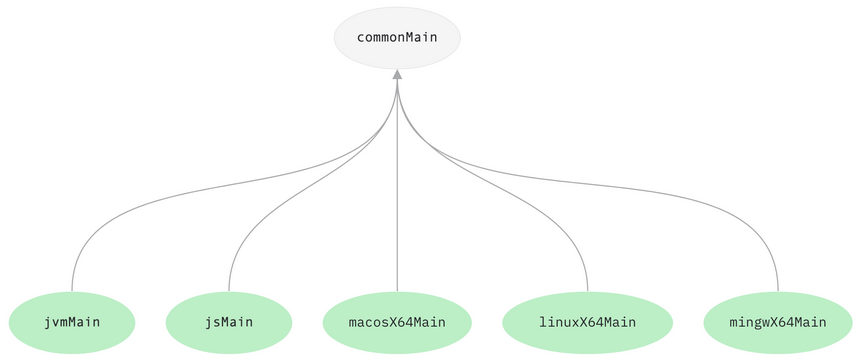
\includegraphics[scale=0.86]{document/chapters/4-collektive/images/km_share_code_on_all_platforms.png}
        \caption{Kotlin Multiplatform sharing code on all platforms}
        \label{fig:km_share_code_on_all_platforms}
    \end{figure}
    \item \textbf{Share code among some platforms}: this organization is usually applied when similar platforms share a big portion of code. As it can be seen in Figure \ref{fig:km_reuse_code}\footref{km_footnote}, it is possible to define hierarchies that allow to organize the shared code, such as the \textit{desktopMain} folder that shares some code with its dependencies, which does not include the whole code present in \textit{commonMain}.
    \begin{figure}[!ht]
        \centering
        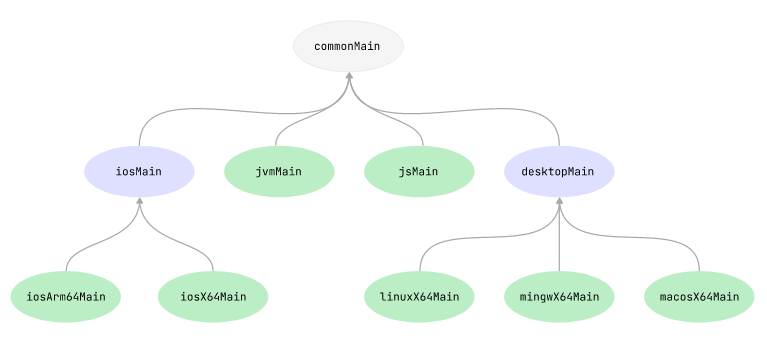
\includegraphics[scale=0.97]{document/chapters/4-collektive/images/kotlin_multiplatform_reuse_code.png}
        \caption{Kotlin Multiplatform reusing code among some platforms of the project}
        \label{fig:km_reuse_code}
    \end{figure}
\end{itemize}

In some cases it might be necessary to access platform-specific APIs from the common code. This can be done by using the specific Kotlin mechanism of expected and actual declarations\footnote{\url{https://kotlinlang.org/docs/multiplatform-connect-to-apis.html} \label{expect_actual_footnote}}.\newline
\begin{figure}[!ht]
    \centering
    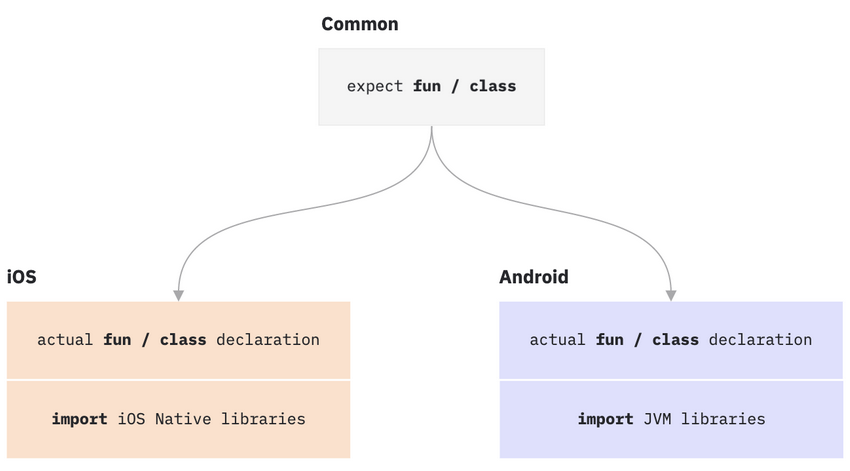
\includegraphics[scale=0.85]{document/chapters/4-collektive/images/km_expect_actual.png}
    \caption{Kotlin Multiplatform expect and actual dependency mechanism}
    \label{fig:km_expect_actual}
\end{figure}
In Figure~\ref{fig:km_expect_actual}\footref{expect_actual_footnote} it is shown an example of this mechanism. For instance, in the common code it is created a new function or class, and it is declared using the keyword \textbf{expect}. The keyword informs the compiler that it should look for the implementation of this element in the platform-specific folders. This can be done by declaring the same function or class by using the \textbf{actual} keyword, which allows taking advantage of platform-specific APIs. In the cited example, the actual implementation required are for the iOS and Android platforms.

Kotlin Multiplatform also includes tools to help developers manage their codebase, such as Gradle plugins that allow for building and testing code across multiple platforms.

One advantage of Kotlin Multiplatform is, for example, the ability to share code between Android and iOS. This can be especially valuable for companies that want to develop apps for both platforms, as it can help reduce development time and costs. With Kotlin Multiplatform, developers can write shared code for common features, such as user authentication or data storage, and then write platform-specific code for the UI and other platform-specific features.

Concluding, Kotlin Multiplatform is the perfect technology to achieve this thesis project, because it allows creating a unique code base that is possible to use on three different platforms: JVM, JavaScript and Native. Moreover, the implementation of platform-specific behaviors is not required, meaning that only the common code has been developed.

\section{Project structure}\label{section:project_structure}
Collektive has been developed as a Gradle project composed by three different submodules, as shown in Figure~\ref{fig:collektive_package_diagram}.
\begin{figure}[!ht]
    \centering
    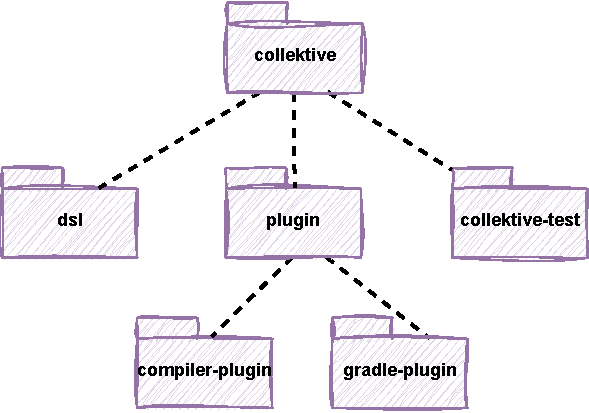
\includegraphics[scale=1.1]{document/chapters/4-collektive/images/collektive_package_diagram.pdf}
    \caption{Package diagram of Collektive project}
    \label{fig:collektive_package_diagram}
\end{figure}
The cited submodules are:
\begin{enumerate}
    \item \textbf{plugin}: it is divided in two submodules itself: 
    \begin{enumerate}
        \item \textbf{gradle-plugin}: necessary plugin used by a gradle project in order to include the compiler plugin. Its structure has been introduced previously in Section~\ref{section:gradle_plugin};
        \item \textbf{compiler-plugin}: the compiler plugin is used to modify a data structure, which to keep tracks of the stack at runtime. For each aggregate function and branch construct, the stack data structure is updated in order to allow the alignment whenever necessary. The specific functionalities of the compiler plugin have been explained in depth in Section~\ref{section:compiler_plugin_solution}; 
    \end{enumerate}
    \item \textbf{dsl}: the actual DSL implementation in Kotlin Multiplatform, where the logic is implemented and that exposes the operators of the aggregate computing. The description of this submodule is going to be presented in Section~\ref{section:dsl};
    \item \textbf{collektive-test}: this submodule is used to test an aggregate program by running it on a simulated environment provided by the Alchemist Simulator~\cite{alchemist}. More details about this are in Section~\ref{section:validation}.
\end{enumerate}

\section{DSL}\label{section:dsl}
A \textbf{DSL} (Domain-Specific Language)\footnote{\url{https://www.jetbrains.com/mps/concepts/domain-specific-languages/}} is a programming language or language construct that is designed to be highly specific to a particular domain, or problem space. Unlike general-purpose programming languages, which are intended to be applicable across a wide range of domains and problem types, DSLs are created to meet the specific needs of a particular application or system. For this reason, general-purpose languages, such as Java, are generally more complex than DSLs.\newline 
DSLs can be implemented in a number of ways, including: standalone programming languages, libraries that extend existing programming languages, or annotations or macros that modify the syntax or behavior of an existing language. DSLs can be used to provide a higher level of abstraction over complex systems or processes, allowing developers to express ideas and concepts in a more concise and intuitive way.\newline
To ensure that DSLs are fit for their intended purpose, they are typically developed in close collaboration with domain experts. In fact, many DSLs are not designed to be used by programmers, but rather by non-technical individuals who are knowledgeable in the relevant domain. This collaborative approach helps to ensure that the DSL is intuitive and expressive for its intended users, allowing them to more easily and effectively express complex ideas and processes.

The DSL developed for this project is organized as shown in the package diagram in Figure~\ref{fig:dsl_packege_diagram}.\newline
\begin{figure}[!ht]
    \centering
    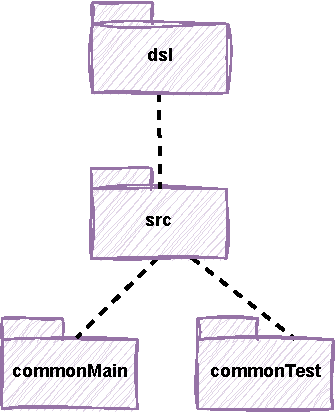
\includegraphics[scale=1]{document/chapters/4-collektive/images/dsl_package_diagram.pdf}
    \caption{Package diagram of Collektive DSL}
    \label{fig:dsl_packege_diagram}
\end{figure}
As previously described, Kotlin Multiplatform allows to create common code that is then compiled on three different targets, which are JVM, JavaScript and Native. Since the behavior of the DSL does not require platform-specific features, it is present in the project only the \textbf{commonMain} package, which contains the whole implementation.\newline
It is also present the \textbf{commonTest} folder, which is used to define the tests to verify the correct behavior of the system and that is possible to run over the different platforms, to ensure that the implementation works as predicted for all the targets. In Section~\ref{section:validation} are going to be presented more details about the tests.

\begin{figure}[!ht]
    \centering
    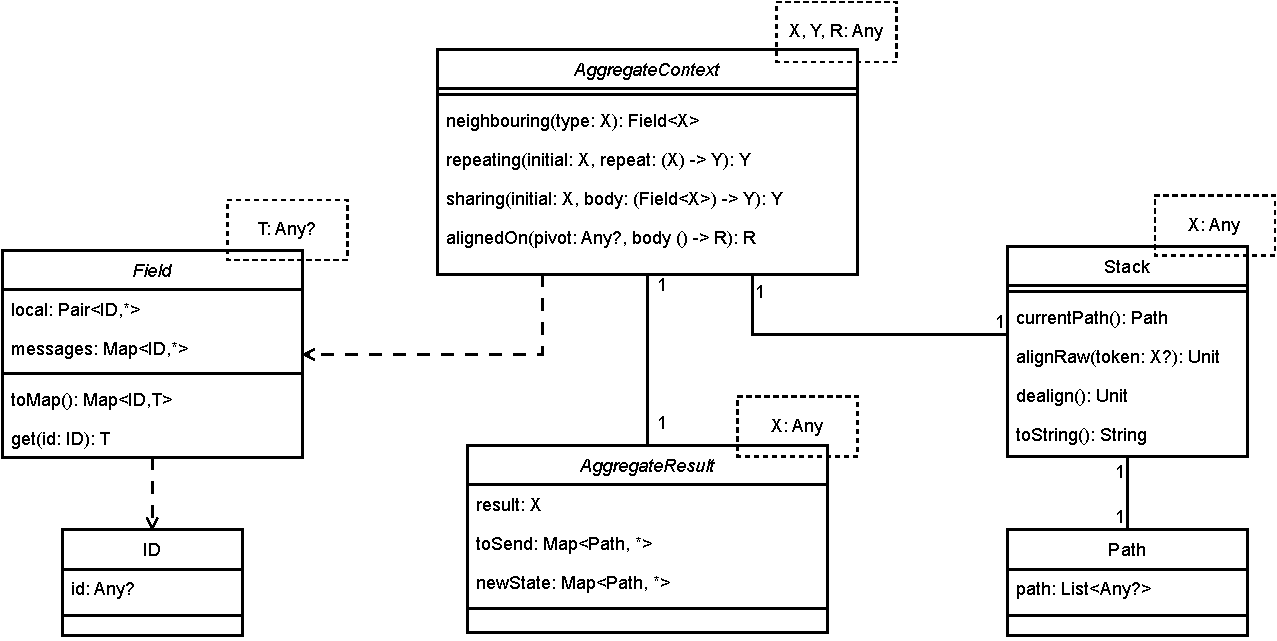
\includegraphics[scale=0.73]{document/chapters/4-collektive/images/dsl_class_diagram.pdf}
    \caption{Class diagram of Collektive DSL}
    \label{fig:dsl_class_diagram}
\end{figure}
The implementation of the project involves the elements presented in the class diagram in Figure~\ref{fig:dsl_class_diagram}, which are:
\begin{itemize}
    \item \textbf{AggregateContext}: it is the class that contains the implementation of the aggregate programming constructs and the function that performs the alignment. Moreover, this class is used to handle all the data necessary for the computation: it stores the local state of the device computed in the previous round, the messages received from the neighbors, the device identifier, and an instance of the stack used to keep track of the computational state. The \textit{AggregateContext} contains also the data class \textit{AggregateResult}, making it possible to instantiate it when the context receiver is \textit{AggregateContext};
    \item \textbf{AggregateResult}: the computation of an aggregate program returns as output an \textit{AggregateResult}, which contains the results obtained from the current iteration, and it is composed by: the actual result returned by the aggregate program, the messages to send to the neighbors to notify them of the current results, and the new device local state;
    \item \textbf{Field}: this class represents the \textbf{computational field}, and it is used by the aggregate constructs to handle this data structure. It contains the local value of the device that is computing and all the messages received by the neighbors. Specifically, the local value is a pair that contains the ID and a map of paths and computed values. Similarly, the messages are composed by the identifier of the neighbor and the same map containing the path and the registered result obtained in the computation corresponding to that path;
    \item \textbf{ID}: a simple identifier which goal is to be able to uniquely recognize different computational device in the aggregate system. Any type of identifier can be used;
    \item \textbf{Stack}: this is the data structure discussed previously in Section~\ref{section:compiler_plugin_solution}, and it is used by the compiler plugin to save the current computational state in order to provide the alignment feature. Through an instance of this class it is possible to retrieve the current path in order to create a computational field or to get the neighboring devices values computed on that specific path;
    \item \textbf{Path}: the path class has already been introduced in Section~\ref{section:compiler_plugin_solution}, and its role is to return an immutable list whenever it is necessary to retrieve the current stack state.
\end{itemize}

A key aspect of this project is the implementation of the aggregate programming constructs contained in the \textit{AggregateContext} class.\newline
The implementation of the \textbf{neighboring} function is reported in Listing~\ref{code:neighboring_implementation}. It accepts in input any parameter, which is the value computed by the current device and that is going to be shared with the neighborhood.
\begin{lstlisting}[caption={Neighboring implementation}, captionpos=b, language=Kotlin, label={code:neighboring_implementation}]
fun <X> neighboring(type: X): Field<X> {
    toBeSent[stack.currentPath()] = type
    val messages = messagesAt(stack.currentPath())
    return FieldImpl(Pair(localId, type), messages)
}
\end{lstlisting}
The behavior of this construct consists on:
\begin{itemize}
    \item Saving the value computed and the current stack in order to send the message to the neighbors;
    \item Retrieving the messages of the neighbors that correspond to the current path;
    \item Finally, returning a field with the local value and the neighbors values, ready to be manipulated.
\end{itemize}

\begin{lstlisting}[caption={Repeating implementation}, captionpos=b, language=Kotlin, label={code:repeating_implementation}]
fun <X,Y : Any> repeating(initial: X, repeat: (X) -> Y): Y {
    val res = 
        if (previousState.containsKey(stack.currentPath())) {
            repeat(previousState[stack.currentPath()] as X) 
        } else {
            repeat(initial)
        }
    state[stack.currentPath()] = res
    return res
}
\end{lstlisting}
The \textbf{repeating} function is used to represent the time evolution, and it allows the field to change dynamically.\newline
This expression needs two parameters:
\begin{enumerate}
    \item \textbf{initial}: the initial value used whenever the function is evaluated for the first time;
    \item \textbf{repeat}: the function that is going to be computed and that takes as input the initial value or the output of the previous round evaluation.
\end{enumerate}
The body of \textit{repeating} can be broken down in the following steps:
\begin{itemize}
    \item It checks whether a previous state exists for the current path in the \textit{perviousState} map;
    \item If a previous state exists, it is invoked the \textit{repeat} function with the value associated with the current path in the previous round;
    \item If a previous state does not exist, the function invokes \textit{repeat} with the \textit{initial} value;
    \item Furthermore, the result of the \textit{repeat} evaluation is stored in the \textit{state} map associated to the current state. This creates the evolution of the local device state, that is going to be used in the next aggregate program iteration;
    \item Finally, the computed value returned by \textit{repeat} is returned.
\end{itemize}

The last aggregate programming constructs is \textbf{sharing}, and its implementation is shown in Listing~\ref{code:sharing_implementation}. As described before in Section~\ref{section:aggregate_programming_introduction}, the \textit{sharing} allows to observe the
neighbors' field, updated the local values and share immediately the updated state in a
single operation.\newline
This function accepts two parameters:
\begin{enumerate}
    \item \textbf{initial}: similarly to the \textit{repeating} constructs, the initial value is used whenever a \textit{sharing} function is evaluated for the first time;
    \item \textbf{body}: it is used to transform immediately the field, resulting a value that is going to be shared with the neighborhood.
\end{enumerate}
The behavior of the \textit{sharing} function can be described as follows:
\begin{itemize}
    \item The function retrieves the messages of the neighbors for the current path from the stack instance;
    \item It checks whether a previous state exists for the current path, similarly to the \textit{repeating} function;
    \item If a previous state exists, the function retrieves it from the \textit{previousState} map. Otherwise, it is used the \textit{initial} value;
    \item Taken the retrieved value, whether it is the \textit{initial} value or the one computed in the previous round, and the messages from the neighbors, a new field instance is created;
    \item The expression invokes the \textit{body} function with the new created field as argument;
    \item The returned value of the \textit{body} function is stored in the \textit{toBeSent} map assigned to the current path. This map contains all the messages to send to the neighbors before the next round begin;
    \item Finally, the output value of \textit{body} is returned by the \textit{sharing} function.
\end{itemize}
\begin{lstlisting}[caption={Sharing implementation}, captionpos=b, language=Kotlin, label={code:sharing_implementation}]
fun <X, Y: Any?> sharing(
    initial: X,
    body: (Field<X>) -> Y
): Y {
    val messages = messagesAt(stack.currentPath())
    val previous = 
        if (previousState.containsKey(stack.currentPath())){
            (previousState[stack.currentPath()]) 
        } else {
                initial
        }
    val subject = FieldImpl<X>(
        Pair(localId, previous), 
        messages
    )
    return body(subject).also {
        toBeSent[stack.currentPath()] = it
    }
}
\end{lstlisting}

The main entry point of an aggregate program is shown in the code in Listing~\ref{code:aggregate_entry_point}.
\begin{lstlisting}[caption={Aggregate entry point}, captionpos=b, language=Kotlin, label={code:aggregate_entry_point}]
fun <X> aggregate(
    localId: ID = IntId(),
    messages:Map<ID,Map<Path,*>>=emptyMap<ID,Map<Path,Any>>(),
    state: Map<Path,*> = emptyMap<Path, Any>(),
    init: AggregateContext.() -> X
) = singleCycle(localId, messages, state, compute = init)
\end{lstlisting}
The \textit{aggregate} function accepts four parameters:
\begin{enumerate}
    \item \textbf{localId}: it is the identification number of a device, which can be used when it is necessary to make the same device compute another round of the aggregate program. This parameter is not mandatory, and, in case it is not defined, a new random identifier is generated;
    \item \textbf{messages}: it might be sometime necessary to give the aggregate program some contextual information about the previous round outcome. This parameter is used to provide the messages received from the neighbors, and it is initialized ad an empty map as default value;
    \item \textbf{state}: similarly to the \textit{messages} parameter, this is used to propagate the previous state of the device in the current round. It is not mandatory, and it is initialized as an empty map whenever it is not found;
    \item \textbf{init}: it is a lambda expression that takes an instance of \textit{AggregateContext} as a receiver object.\newline
    A lambda expression is a block of code that can be executed later, and it can be passed around as a value. In Kotlin, lambda expressions can have a receiver object, which is an object on which the lambda is invoked.\newline
    In Kotlin, a context receiver is a way of providing a context or a scope to a block of code, such as a lambda expression. A context receiver allows the block of code to access the properties and functions of the receiver object using the \textit{this} keyword, without having to explicitly specify the receiver object in the code.\newline
    This means that when the lambda expression \textit{init} is invoked, it has access to the properties and functions of the \textit{AggregateContext} object. By using the aggregate function, it is then possible to define the lambda that is going to be computed, and, by doing so, the aggregate constructs defined in the \textit{AggregateContext} can be used freely.
\end{enumerate}

This \textit{aggregate} function in Listing \ref{code:aggregate_entry_point} allows the computation of a single cycle, which means that only one round is going to be performed. This requires the user of the DSL to define how the different devices should communicate.\newline
In Section~\ref{section:validation} it is going to be presented a different \textit{aggregate} function that allows to run multiple rounds of an aggregate program, used to test the correct behavior during the validation process.

The \textit{singleCycle} function returns an \textbf{AggregateResult}, which is the output of an aggregate program in Collektive. The implementation of the \textit{singleCycle} function is reported in Listing~\ref{code:single_cycle_return_type}. This class contains the value computed from the aggregate lambda, a map of all the messages to send to the neighbors, and the new state of the device.
\begin{lstlisting}[caption={Single cycle \textit{AggregateResult} output}, captionpos=b, language=Kotlin, label={code:single_cycle_return_type}]
with(AggregateContext(localId, messages, state)) {
    AggregateContext.AggregateResult(
        compute(),
        messagesToSend(),
        newState()
    )
}
\end{lstlisting}

\section{Usage example}\label{section:usage_example}
One important aspect to consider during the development of a DSL is its usability. It is important to provide the user with a minimal set of operators, each of them with a clear purpose.\newline
This is what has been achieved with Collektive, since the constructs are coherent with the aggregate programming original operators.

In order to use Collektive, it is necessary to perform some steps to set up the environment:
\begin{enumerate}
    \item \textbf{Include the compiler plugin}: since the alignment is crucial for the DSL to work, it is important to include into the Gradle project the custom Gradle plugin created to expose the Kotlin compiler plugin.\newline
    Whenever a new submodule of Collektive is created, the Gradle plugin can be included as shown in the code in Listing~\ref{code:include_gradle_plugin};
\begin{lstlisting}[caption={Inclusion of the custom Gradle plugin to a local Gradle submodule}, captionpos=b, language=Kotlin, label={code:include_gradle_plugin}]
plugins {
    id("io.github.elisatronetti.kotlinAlignmentPlugin") version "0.1.0"
}
\end{lstlisting}
    \item \textbf{Include the DSL}: it is also necessary to include the DSL to the project, in order to be able to access all the aggregate programming constructs developed. The code in Listing~\ref{code:include_dsl} shows how to include it into a new Collektive submodule.
\begin{lstlisting}[caption={Inclusion of the DSL to a local Gradle submodule}, captionpos=b, language=Kotlin, label={code:include_dsl}]
dependencies {
    implementation(project(path=":dsl"))
}
\end{lstlisting}
\end{enumerate}

Once the setup is finished, the DSL is available into the new submodule. By calling the function \textbf{aggregate}, the DSL functions \textbf{neighboring}, \textbf{repeating} and \textbf{sharing} can be used. Moreover, the compiler plugin included provides the correct alignment of the elements.
\begin{lstlisting}[caption={Example of an aggregate program developed with Collektive}, captionpos=b, language=Kotlin, label={code:aggregate_program_example}]
val double: (Int) -> Int = { it * 2 }
val testValue: Int = 2
aggregate {
    neighboring(double(testValue))
}
\end{lstlisting}
The snippet of code in Listing~\ref{code:aggregate_program_example} shows an example of usage. The program shares with the neighbors the double of a local number. In this example, the value of the number is hardcoded, but in a real world example, this value might depend on the device environment, which would make different devices have a different value evaluation.

\section{Validation}\label{section:validation}
The term validation refers to the process of ensuring that the software meets the intended requirements and specifications and fits for its intended use. Validation is a critical aspect of the software development process as it helps to ensure that the software is free of defects, meets the expectations of its users, and performs its intended function correctly.

The validation process typically involves testing the software in various ways, and the goal of each type of testing is to ensure that the software meets the intended goal and that it performs as expected in various environments and scenarios.

Collektive validation consists on two main tests:
\begin{enumerate}
    \item \textbf{Functional testing}: involves verifying that the software performs its intended functions correctly and without errors;
    \item \textbf{Compatibility testing}: involves testing the software's ability to operate correctly in different environments and with different hardware and software configurations.
\end{enumerate}
These validation processes are achieved in two different ways, which are going to be discussed in this section.

The first method tests both the functionalities and the compatibility of the system. This is obtained by taking advantage of the Kotlin Multiplatform features because, when it comes to testing, it provides several tools and frameworks that can be used to test code written in Kotlin on different platforms.\newline
One popular testing framework for Kotlin Multiplatform is \textbf{KotlinTest}\footnote{\url{https://kotlinlang.org/docs/multiplatform-run-tests.html}}; said framework is a multiplatform testing library that provides a common API for writing tests that can be run on different platforms. It supports a range of testing styles, including behavior-driven development (BDD) and property-based testing.\newline
Kotlin Multiplatform also provides a set of common annotations that can be used to mark tests and test suites, such as the \textbf{@Test} annotation. These annotations can be used in conjunction with testing frameworks like \textit{KotlinTest} to write and run tests on multiple platforms.\newline
Since the DSL is developed using Kotlin Multiplatform, the package \textbf{commonTest} contains the test implemented using \textit{KotlinTest}.\newline
\begin{figure}[!ht]
    \centering
    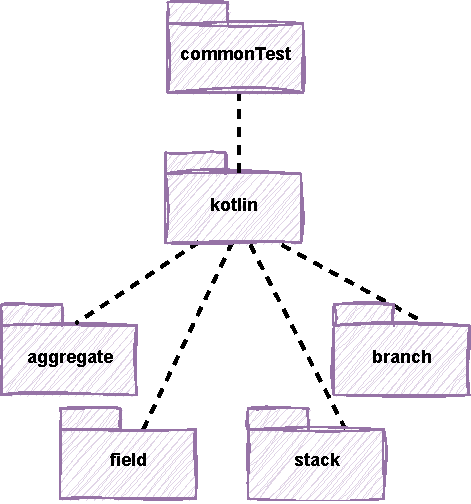
\includegraphics[scale=1.1]{document/chapters/4-collektive/images/common_test_package_diagram.pdf}
    \caption{Package diagram of Collektive DSL tests}
    \label{fig:common_test_package_diagram}
\end{figure}
The organization of the folder \textit{commonTest} is shown in Figure~\ref{fig:common_test_package_diagram}. It contains only the \textbf{kotlin} subfolder, since the implementation of platform-specific tests is not required.\newline
The test are organized in the following folder system:
\begin{itemize}
    \item \textbf{field}: contains unit testing of the \textit{Field} class and the field manipulation functions, such us the retrieval of the lower comparable value contained in the field;
    \item \textbf{stack}: similarly to the \textit{Field}, also the \textit{Stack} class requires unit testing, to verify that it works as predicted;
    \item \textbf{branch}: it contains all the possible testing of the branching alignment. It verifies the correct alignment of simple if, else-if and else blocks and expressions. Furthermore, it tests the alignment of the \textit{when} Kotlin expressions;
    \item \textbf{aggregate}: finally, in this folder are contained all the tests of the aggregate programming constructs, which are \textit{neighboring}, \textit{repeating} and \textit{sharing}.
\end{itemize}

Since testing only one round of an aggregate program would not be enough to ensure the correct system behavior, it has been implemented an infrastructure that allows to test multiple rounds.\newline
It is necessary to create a class that allows to save the messages and deliver them to other devices. This class is called \textbf{Network}, and its interface is shown in the code in Listing~\ref{code:network_interface}.
\begin{lstlisting}[caption={Network interface to simulate multiple round of an aggregate program in tests}, captionpos=b, language=Kotlin, label={code:network_interface}]
interface Network {
    fun send(localId: ID, message: Map<Path, *>)
    fun receive(): Map<ID, Map<Path, *>>
}
\end{lstlisting}
Before creating an aggregate program, it is necessary to instantiate a \textit{Network}, which contains an internal map of messages, and it is used to handle the communication between devices.

It is also necessary to create a new entry point for the DSL, which makes it possible to accept parameters to handle multiple rounds.

\begin{lstlisting}[caption={Aggregate programming entry point used to compute multiple rounds}, captionpos=b, language=Kotlin, label={code:aggregate_entry_point_for_multiple_rounds}]
fun <X> aggregate(
    condition: () -> Boolean,
    network: Network = NetworkImpl(),
    init: AggregateContext.() -> X
) = runUntil(condition, network, compute = init)
\end{lstlisting}

The new \textit{aggregate} function is reported in Listing~\ref{code:aggregate_entry_point_for_multiple_rounds}, and it accepts the following parameters:
\begin{enumerate}
    \item \textbf{condition}: it is a lambda expression that takes no arguments and returns a \textit{Boolean} value, which is used to establish whether the computation should run another round or not;
    \item \textbf{network}: an instance of the \textit{Network} class introduced in the code in Listing~\ref{code:network_interface}, which is used to handle sending and receiving messages;
    \item \textbf{init}: the actual aggregate program, contained in a lambda expression which has as receiver object an \textit{AggregateContext}.
\end{enumerate}

This \textit{aggregate} function calls \textbf{runUntil},  and in the snippet of code in Listing \ref{code:run_until_body} it is reported the main logic its implementation.
\begin{lstlisting}[caption={Main logic of the \textit{runUntil} function}, captionpos=b, language=Kotlin, label={code:run_until_body}]
while (condition()) {
    computed = singleCycle(
        localId,
        network.receive(),
        state,
        compute
    )
    state = computed.newState
    network.send(localId, computed.toSend)
}
\end{lstlisting}

The purpose of \textit{runUntil} is to repeatedly execute the \textit{compute} lambda expression until the \textit{condition} lambda returns \textit{true}.\newline
In order to do that, every time it is necessary a new iteration, it is computed a \textbf{singleCycle}, which is the same function used in the normal aggregate program execution, which was presented in Section~\ref{section:dsl}. A cycle requires the local identifier of the device, it retrieves from the network the message received from the neighbors, the current local state of the device and the lambda that define the computation.\newline
Afterwords, it updates the local state, and it sends the via network the messages regarding the computed values of this round.

By using the mechanisms just presented, it is possible to create tests that check the correct interaction between devices, also verifying that the alignment works properly. Moreover, \textit{KotlinTest} allows to run the implemented tests over the different targets of the project, testing the compatibility of the software over different platforms.

The second validation process regards mainly the functional testing, and it aims to provide a proof of concept of the potential of Collektive.\newline
The goal is to implement a gradient algorithm using the constructs provided by the DSL, and then simulate the computation of a distributed system using \textbf{Alchemist Simulator}~\cite{alchemist}.\newline
In order to achieve this objective, it has been created a new submodule in the Collektive project called \textbf{collektive-test}. Alchemist dependencies, the DSL, and the Gradle and compiler plugin are fundamental for this purpose. 

The following classes are required in order to create the correct infrastructure used to make the simulation possible:
\begin{itemize}
    \item \textbf{CollektiveDevice}: this is the abstraction of a node present in the simulation environment. This class makes possible to send and receive messages, to store neighbors information and to uniquely identify nodes;
    \item \textbf{CollektiveIncarnation}: an incarnation is the interpreter that allows Alchemist to understand a language and to execute it correctly. This incarnation is specific for Collektive, and it is used to find the aggregate entry point through reflections, and it defines how each iteration of the aggregate program should be performed.
\end{itemize}

The algorithm is implemented as an \textit{AggregateContext} extension function, and it is shown in the code in Listing~\ref{code:gradient_algorithm}.
\begin{lstlisting}[caption={Gradient algorithm implemented using Collektive}, captionpos=b, language=Kotlin, label={code:gradient_algorithm}]
fun AggregateContext.gradient(
    source: Boolean,
    sensor: DistanceSensor
) = sharing(Double.POSITIVE_INFINITY) { distances ->
    val paths: Field<Double> = sensor.distances() + distances
    val minByPath = paths.min(includingSelf = false)?.value
    when {
        source -> 0.0
        minByPath == null -> Double.POSITIVE_INFINITY
        else -> minByPath
    }
}
\end{lstlisting}
The algorithm calculates the gradient from a node that is defined as \textit{source}. By using the \textit{sharing} construct, it is possible to retrieve all the neighbors' data. This is used to obtain the distances of the neighbors from the source, and then, the distance of the current device is added to the neighbors one. After that, it is searched the minimum distance, which is going to be the current distance from the device to the source node. Finally, the algorithm returns zero if the node is the source, infinity if the minimum distance is not found, or the minimum value.\newline
Since \textit{sharing} has been used, the computed value is then propagated to the neighborhood.

In order to make the incarnation find the aggregate program, it is necessary to define an entry point, which is reported in the code in Listing~\ref{code:gradient_algorithm_entry_point}.
\begin{lstlisting}[caption={Gradient algorithm entry point}, captionpos=b, language=Kotlin, label={code:gradient_algorithm_entry_point}]
class Aggregate(private val node: CollektiveDevice<*>) {
    private val nodeId = node.node.id
    private var state = emptyMap<Path, Any?>()
    fun entrypoint() = aggregate(
        IntId(nodeId), 
        node.receive(),
        state
    ){
        gradient(nodeId == 0, node)
    }.also { state = it.newState }
}
\end{lstlisting}
The \textbf{Aggregate} class takes as parameter a \textit{CollektiveDevice}, which is used to establish the device that is currently computing.\newline
The function \textbf{entrypoint()} is the function that the incarnation is going to look for and execute.\newline
The entry point creates an \textit{aggregate} block, which takes as parameter all the contextual information about the device: the device identifier, the messages received from the neighbors, and the state obtained in the previous round. The computation consists of the execution of the gradient algorithm just presented, and it also defines that the node with the identification number \textit{0} is going to be the source.\newline
At the end of the single execution of the aggregate program, the current state of the device is updated.

Finally, it has been created the simulation environment, which creates \textbf{200 nodes} in a 2D space. The result of the creation of the nodes is shown in Figure~\ref{fig:collektive_before_running_the_simulation}.
\begin{figure}[!ht]
    \centering
    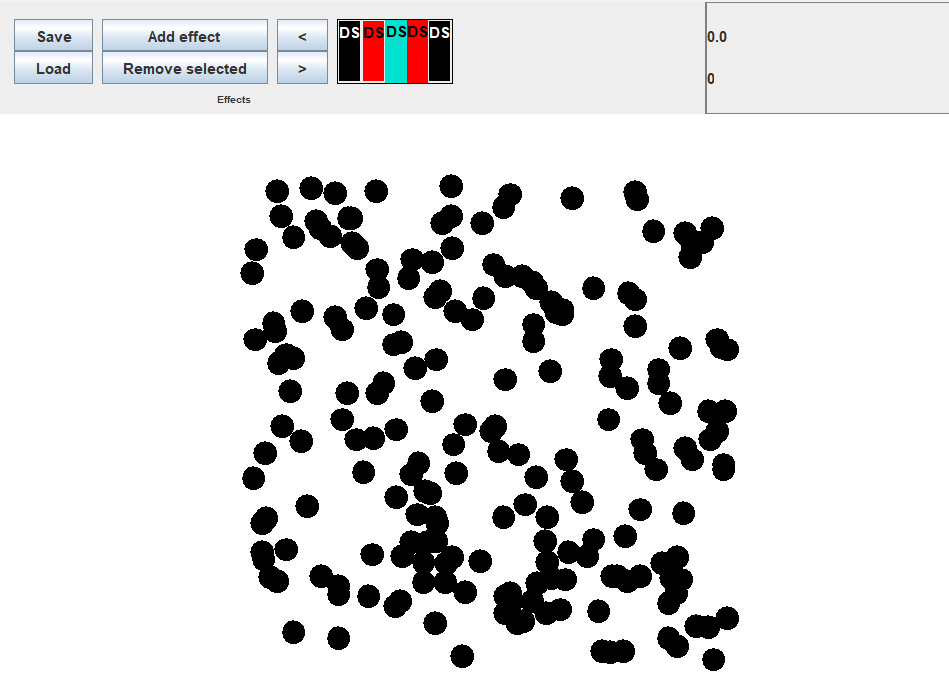
\includegraphics[scale=0.75]{document/chapters/4-collektive/images/collektive_before_running_the_simulation.png}
    \caption{Alchemist simulation environment before running Collektive gradient algorithm}
    \label{fig:collektive_before_running_the_simulation}
\end{figure}

Once Alchemist has generated the nodes that are going to be involved, it is only necessary to run the simulation. The UI of Alchemist is going to color differently the nodes, basing on the distance from the source: the more the node is colored in red, the more is near to the source, the more the color tends to a colder color, the further is from the source node.\newline
The source node can be distinguished from the other nodes from the different shape and color: it is shaped as a square, and it has a light blue border.

The user interface of the Alchemist Simulator shows also other information:
\begin{enumerate}
    \item \textbf{Rounds performed}: it refers to the number of time the aggregate program has been executed before reaching a stable gradient. The example showed in Figure~\ref{fig:collektive_simulation_completed} performed \textbf{30331} rounds;
    \item \textbf{Execution time}: this is a valuable indicator of the performance of the algorithm written using Collektive. The example in exam found a stable solution of the gradient in \textbf{150.73 milliseconds}.
\end{enumerate}
\begin{figure}[!ht]
    \centering
    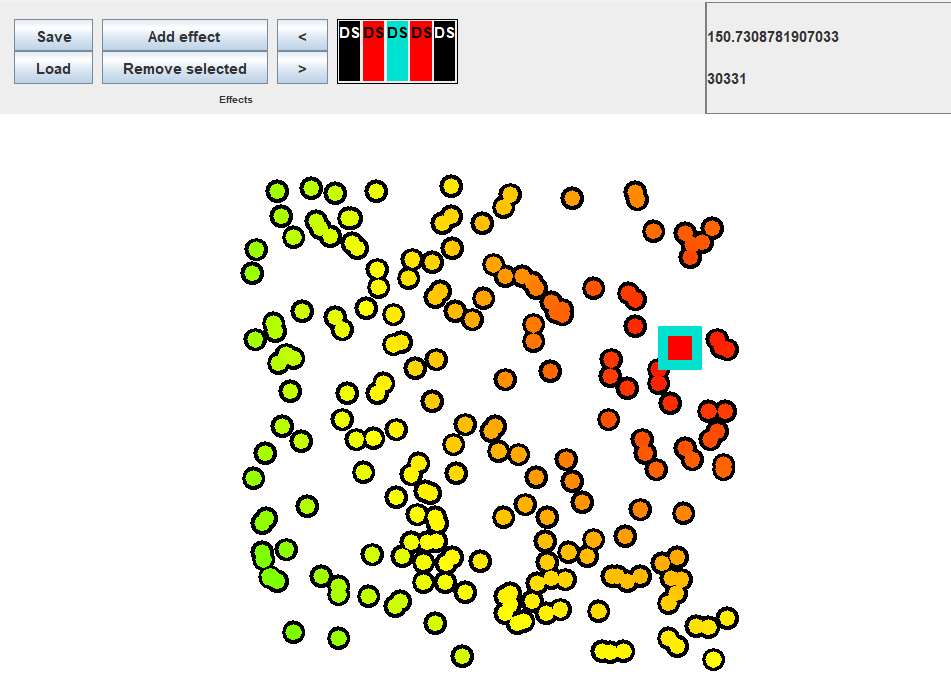
\includegraphics[scale=0.75]{document/chapters/4-collektive/images/collektive_simulation_completed.png}
    \caption{Alchemist simulation environment execution of Collektive gradient algorithm}
    \label{fig:collektive_simulation_completed}
\end{figure}

This validation process using Alchemist Simulator shows the potential of Collektive: it is easy to implement algorithms that define the behavior of a system, and the execution is fast and reliable.